\documentclass{l4proj}
\usepackage{blindtext}
\usepackage[backend=biber, sorting=nyt, style=apa]{biblatex}
\usepackage{hyperref}
\addbibresource{dissertation.bib}

\providecommand{\tightlist}{%
  \setlength{\itemsep}{0pt}\setlength{\parskip}{0pt}}

\title{A Deep Learning Approach to Musical Effects}
\author{Kieran McCool}

\begin{document}

\maketitle

\tableofcontents
\hypertarget{introduction}{%
\chapter{Introduction}\label{introduction}}

\hypertarget{musical-effects}{%
\section{Musical Effects}\label{musical-effects}}

Musical effects are transformations which can be applied to an audio
track to change the sound in some way. These can take the form of simple
tweaks to the frequency range of the track to applying pitch modulation
and beyond.

Musical effects can completely change the way a track sounds and the art
of mixing a track is - in many ways - more complicated than the
composition and performance of the track. Sound engineers have a huge
range of choices and responsibility when it comes to getting the
soundscape correct for the final product.

The music industry is one of the few domains which is still to fully
embrace digital technology. Many recording studios and musicians still
make use of analogue equipment such as tape, vinyl, and vacuum tubes. As
these technologies become more outdated and niche, the cost of
maintaining and replacing equipment rises. As such, it is essential that
software modelling catches up to the performance and quality of these
older technologies.

\hypertarget{musical-effect-modelling}{%
\section{Musical Effect Modelling}\label{musical-effect-modelling}}

The main standard for producing digital effects for use with audio is
through the Virtual Studio Technology (VST) protocol. This protocol
defines a standardised definition for how a VST host would behave,
allowing VST Plugins to be created which manipulate or use the audio
track in some way.

The technology itself is fairly flexible and allows everything from
audio visualisation tools to CPU intensive transformations to be
applied. These effects can also be stacked and ordered easily and
intuitively.

Most effects however, are limited to digital signal processing (DSP)
based transformations, the likes of which are unable to replicate the
non-linearity of many analogue methods. This is cause for concern in the
music industry and is the reason many professionals and hobbyists claim
that they are inadequate for anything more than practice and
experimentation.

\hypertarget{machine-learning}{%
\section{Machine Learning}\label{machine-learning}}

In recent years, a huge amount of research has gone into machine
learning. Its application frequently makes news for revolutionising the
various industries it is applied to. As such, it would be interesting to
see the effectiveness of machine learning in this field.

Of particular interest to us were convolutional neural networks and
Long-Short Term Memory (LSTM) networks, which both seem to be at the
forefront of deep learning research. However, the application of machine
learning to audio data is in its infancy, resulting in quite a
challenging implementation with many layers to it and several
dependencies.

The idea of the project is to create two audio tracks, one which is a
clean signal from an instrument and one which is the result of applying
a VST effect to that clean track. We would then create a neural network
which would take samples from the clean signal and be trained to produce
the value of the corresponding sample in the processed track.

\hypertarget{background}{%
\chapter{Background}\label{background}}

\hypertarget{nebula-vst}{%
\section{Nebula VST}\label{nebula-vst}}

Nebula yields the best results current modelling technologies can
achieve. It achieves this using Volterra Kernel Modelling to better
represent non-linear behaviours and exhibiting some level of memory
capacity. This allows it to model time-based effects and non-linearity
more effectively than primitive DSP approaches.

In doing this, it has become one of the most praised pieces of modelling
software, criticised only for its system requirements and its steep
learning curve. Requiring a minimum of 8GB of RAM with a recommended
amount of 16-128GB, it is a rather demanding piece of software.

Given that Nebula is the best plugin available at this time, for this
project to be considered a success, it should be as good as or better
than Nebula.

\hypertarget{project-magenta}{%
\section{Project Magenta}\label{project-magenta}}

Project Magenta is a venture by the Google Brain Team, their goal is to
explore the use of machine learning in creating art, with a particular
interest in music. Most of their research is in audio synthesis with
some ventures into genre classification and similar problems.

However, this project does raise some interesting questions about the
ability of deep learning to characterise the complexities of music.

Most of their work however, was limited to interacting with MIDI data
rather than with raw audio samples, perhaps limiting the complexity of
the problem, making it an unfair comparison in terms of complexity to
effect modelling.

\hypertarget{wavenet}{%
\section{WaveNet}\label{wavenet}}

Another use of deep learning for audio synthesis is in the field of
generating realistic text-to-speech. DeepMind's WaveNet is a generative
network, trained using raw audio samples to predict the value of the
next sample in the series.

The project found that while generally an LSTM is better suited to this
kind of time-series problem, they could achieve similar results using
stacked convolutional layers applying dilated casual convolutions. At
each layer they would double the dilation amount up to a maximum before
starting again at 1. This a increases the receptive field of the network
in a similar way to how an LSTM selectively remembers traits while
maintaining the ease of training of a convolutional network.

Another way in which the WaveNet implementation differs from a standard
convolutional network is in its output layer. Instead of predicting a
sample as a floating point value representing the amplitude, the output
is a one-hot encoded vector where the largest index corresponds with the
\(\mu\)--Law encoded integer of the sample.

\begin{center}

    $F(x) = sgn(x)\frac{ln(1+\mu|x|)}{ln(1+\mu)} -1 <= x <= 1$

    $\mu$ Law as expressed in \LARGE{SOURCE THIS}
\end{center}

This network has proven itself to be capable of generating extremely
effective, almost human sounding text-to-speech and is far easier to
train than a standard LSTM-based approach.

\hypertarget{aims}{%
\chapter{Aims}\label{aims}}

\hypertarget{effect-choices}{%
\section{Effect Choices}\label{effect-choices}}

The aim of this project is to explore the viability and success of deep
learning in effect modelling at a fairly general level. As such, a
multitude of different effects should be tested.

While there is a huge range of commonly used effects, and an even larger
range of different variations of these same effects with subtly
different responses, most of them fit in to one of three groups.

\begin{center}
\begin{tabular}{ |c|c|c| } 
 \hline
    \textbf{Amplitude Based} & \textbf{Frequency Based} & \textbf{Time Based} \\ 
 \hline
 Distortion & High/Low Pass Filter & Chorus \\ 
 Fuzz & Pitch Shift/Octave & Delay \\ 
 Compression & & Reverb \\ 
 Amplifier/Cab Simulation & & \\ 
 \hline
\end{tabular}
\end{center}

Narrowing the scope of the project to include only these effects results
in a good indication of viability across a multitude of effects, while
keeping the project scope at an attainable level.

\hypertarget{deep-learning}{%
\section{Deep Learning}\label{deep-learning}}

Deep learning has demonstrated extreme potential in the realm of
text-to-speech and audio generation. As such, it is possible that it
would prove similarly effective in effect modelling.

A few different types of deep learning were of particular interest. With
regards to amplitude based effects, most of the transformation is
carried out across a narrow time-frame, and non-linearity is limited. As
such, for these effects it was hypothesised that a simple Convolutional
Net with a window of narrow window of samples as the input would be
sufficient. The same was thought for the frequency based effects such as
filters.

For Time Based effects however, the active window of the effect can be
much larger, with reverb sometimes being used with multiple second long
tail. Given that music is generally sampled at 44,100Hz, this means that
for the network to model this, it would require more than 44,100 samples
as its input vector. This is obviously impractical as the memory
requirements and time to train the network would be impractical.

In order to try and work around this, LSTM networks would be explored as
a potential remedy. These would be able to learn which aspects of the
track need to be remembered to best replicate the effect.

\hypertarget{methods}{%
\chapter{Methods}\label{methods}}

\hypertarget{network-architecture}{%
\section{Network Architecture}\label{network-architecture}}

\hypertarget{convolutional-networks}{%
\subsection{Convolutional Networks}\label{convolutional-networks}}

Apart from WaveNet, guidance for creating a network architecture
suitable for capturing the complexities of audio data were hard to come
by. Most of the experience I had with machine learning was limited to
completing example problems and tutorials.

As such, the first goal was to adapt one of these example networks to
receive audio data rather than text or image data which the tutorial
used. The network I chose to adapt was one which performed well on the
MNIST image classification dataset.

This network consisted of 2 Convolutional Layers with Rectified Linear
Unit (ReLU) activation layers between, the results of which were then
forwarded into a Max Pooling layer before a series of fully connected
layers. A simplified diagram of this is shown in Figure \ref{fig:nn}

\begin{figure}
\centering
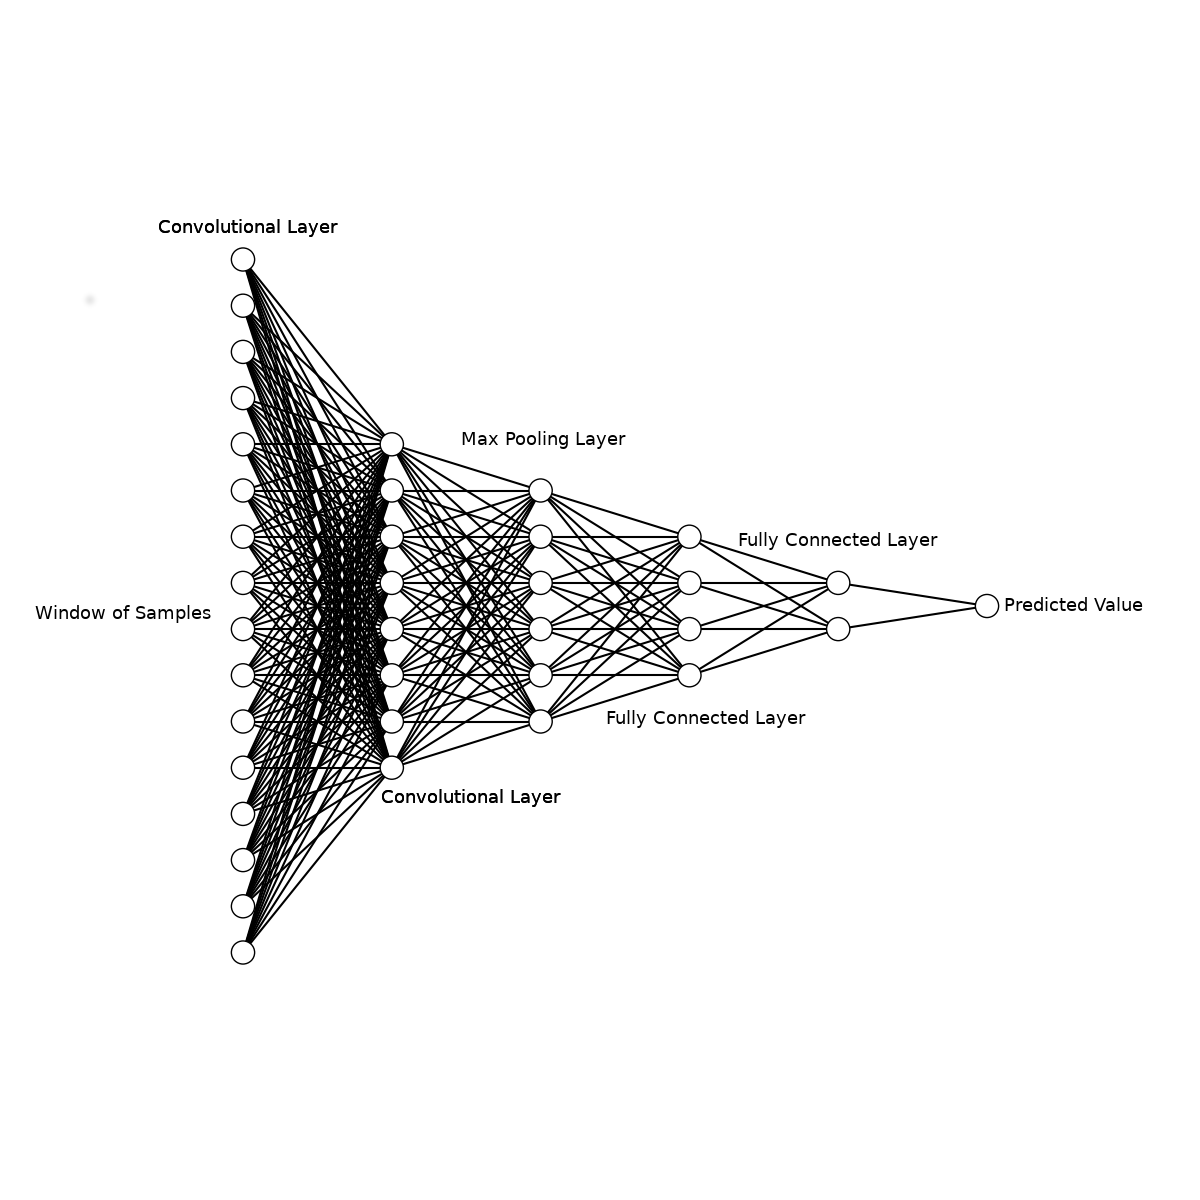
\includegraphics[width=\textwidth,height=6in]{images/cnn.png}
\caption{A Simplified Diagram of the Convolutional Network
used\label{fig:nn}}
\end{figure}

\hypertarget{long-short-term-networks}{%
\subsection{Long-Short Term Networks}\label{long-short-term-networks}}

It was thought that while a convolutional network would be impractical
in learning the spatial elements required to reproduce a time-based
effect such as reverb or chorus. Some kind of recursive neural network
(RNN) was hypothesised to be able to replicate this behaviour as it
would take the samples from the track in one at a time and learn what
properties to remember and for how long.

The downside to this was that training time is much slower as the
network has a great deal more properties to learn than a typical
feed-forward network.

\hypertarget{wavenet-1}{%
\subsection{WaveNet}\label{wavenet-1}}

Another idea was to implement the same basic network as WaveNet. Using
dilated casual convolutions to classify the predicted value based on a
one-hot encoded vector. This worked extremely well for generating speech
data, exhibiting a ``subjective naturalness never before seen.''

\hypertarget{evaluating-success}{%
\section{Evaluating Success}\label{evaluating-success}}

\hypertarget{melspectograms}{%
\subsection{Melspectograms}\label{melspectograms}}

Spectograms are a graphical representation of an audio signal. They show
detailed information about the frequencies present in a signal over
time. The resulting representation is often used in speech recognition
problems as a means of feature extraction. Allowing the system to
identify the words spoken. As such, they can be used as a quantitative
means of evaluating how closely the network output matches the VST
output.

The process for creating Melspectograms is based on mapping the signal
to Mel Scale using the Fourier Transform. This can then be represented
as a heatmap of frequencies in Hz which are present in the audio. Figure
({\textbf{???}}) shows an example of this on an audio track.

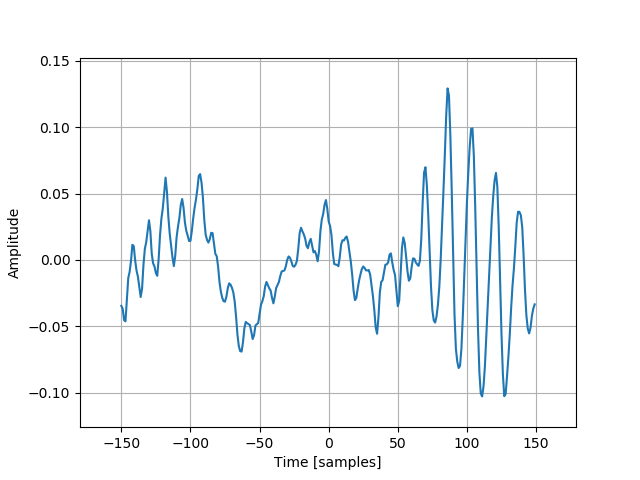
\includegraphics{images/spect.png}\{width=4in keepaspectratio\}

\hypertarget{impulse-response}{%
\subsection{Impulse Response}\label{impulse-response}}

\hypertarget{abx-testing}{%
\subsection{ABX Testing}\label{abx-testing}}

\hypertarget{implementation}{%
\chapter{Implementation}\label{implementation}}

\begin{itemize}
\tightlist
\item
  PyTorch
\item
  SciPy.signal
\item
  LibRosa
\item
  Reaper and the VSTs used
\item
  How the pieces fit together
\end{itemize}

\hypertarget{results}{%
\chapter{Results}\label{results}}

\begin{itemize}
\tightlist
\item
  Split into quantitative and qualitative
\item
  Signal Analysis (Quantitative)
\item
  Spectogram GIFs (Quantitative)
\item
  Loss over time / Standard Deviation of loss ( ??? - Loss hasn't really
  proven to be particularly meaningful)
\item
  ABX tests with classmates/friends (Qualitative)
\end{itemize}

\hypertarget{conclusion}{%
\chapter{Conclusion}\label{conclusion}}

\hypertarget{references}{%
\chapter{References}\label{references}}
\end{document}
